\section{CNN-Approach}

\begin{frame}
    \frametitle{Datasets}
    \begin{enumerate}
        \item byarticle (~600 articles directly labeled; \emph{quality data})
        \item bypublisher (~600k articles indirectly labeled by publisher; \emph{quantity data})
        \item byart-bypub-mix (byarticle + ~1100 articles from bypublisher)
    \end{enumerate}
    due to time and ressource constraints, only byarticle and mix were used, as well as a seed
\end{frame}

\begin{frame}
    \frametitle{Baselines}
    \begin{itemize}
        \item Logistic Regression
        \item SGDClassifier (SVM)
    \end{itemize}
\end{frame}

\begin{frame}
    \frametitle{Logistic Regression}
    \begin{tabular}{l|c|c}
                  & Quality & Mix \\\hline
        Accuracy  & ~80 & ~68 \\
        Precision & ~76 & ~67 \\
        Recall    & ~60 & ~50 \\
        F1        & ~67 & ~57
    \end{tabular}
    consistent results due to the seed
\end{frame}

\begin{frame}
    \frametitle{SVM}
    \begin{tabular}{l|c|c}
                  & Quality & Mix \\\hline
        Accuracy  & ~71-76 & ~63-69\\
        Precision & ~55-64 & ~56-60\\
        Recall    & ~65-80 & ~59-70\\
        F1        & ~60-66 & ~59-65
    \end{tabular}
    inconsistent results despite seed due to Stochastic Gradient Descent
\end{frame}

\begin{frame}
    \frametitle{CNN}
    \begin{tabular}{l|c|c}
                  & Quality & Mix \\\hline
        Accuracy  & ~69-74 & ~59-66 \\
        Precision & ~53-63 & ~51-61 \\
        Recall    & ~47-67 & ~57-72 \\
        F1        & ~52-60 & ~57-61
    \end{tabular}
\end{frame}

\begin{frame}
    \frametitle{Techniques}
    \begin{itemize}
        \item BatchNormalization
        \item Dropout
        \item (Global)MaxPooling
        \item Learning Embeddings and Pre-Learned Embeddings (ELMo/Word2Vec/GloVe)
    \end{itemize}
\end{frame}

\begin{frame}
    \frametitle{CNN Graph}
    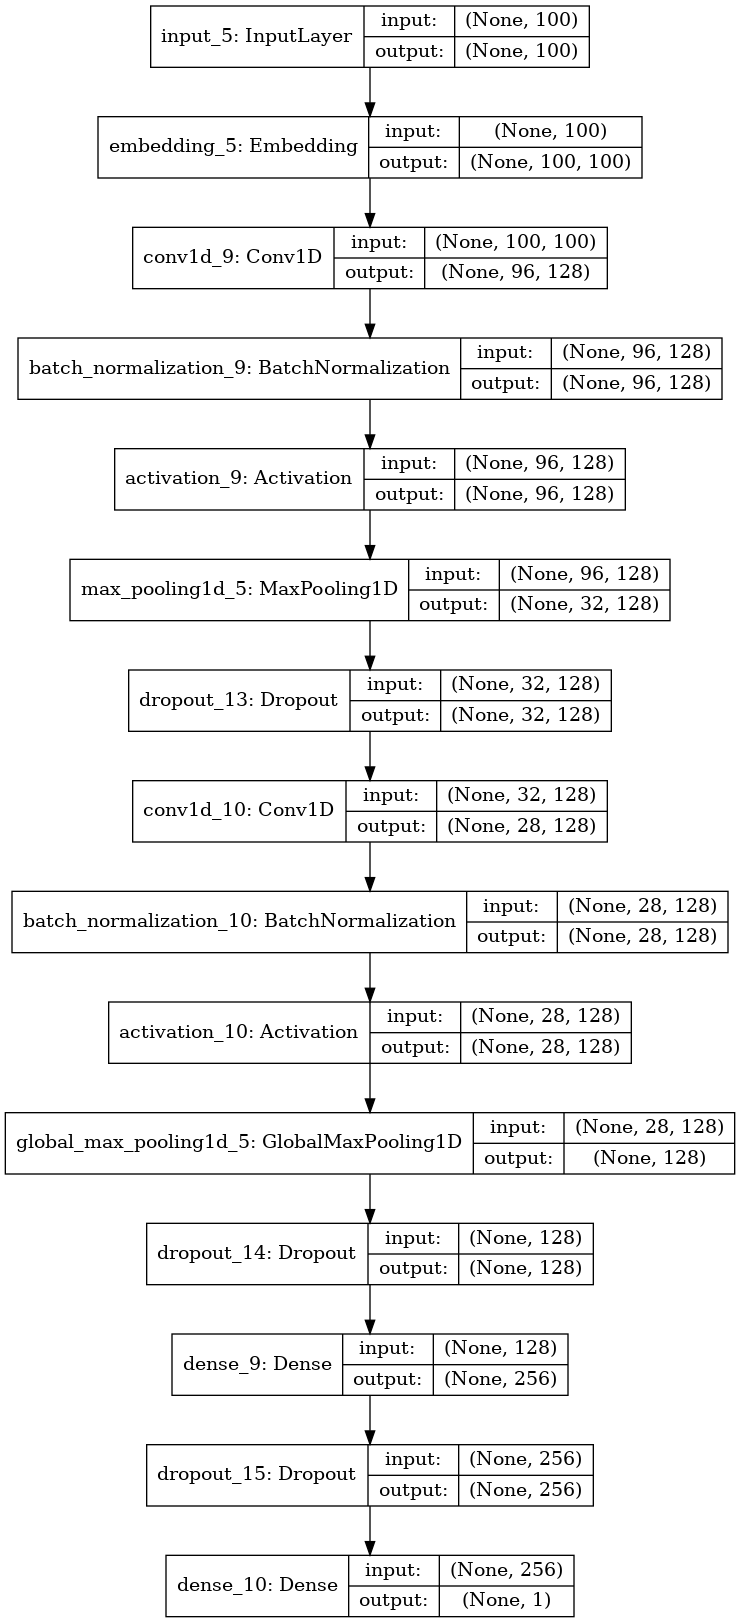
\includegraphics{cnn_model.png}
\end{frame}

\begin{frame}
    \frametitle{ELMo Model}
    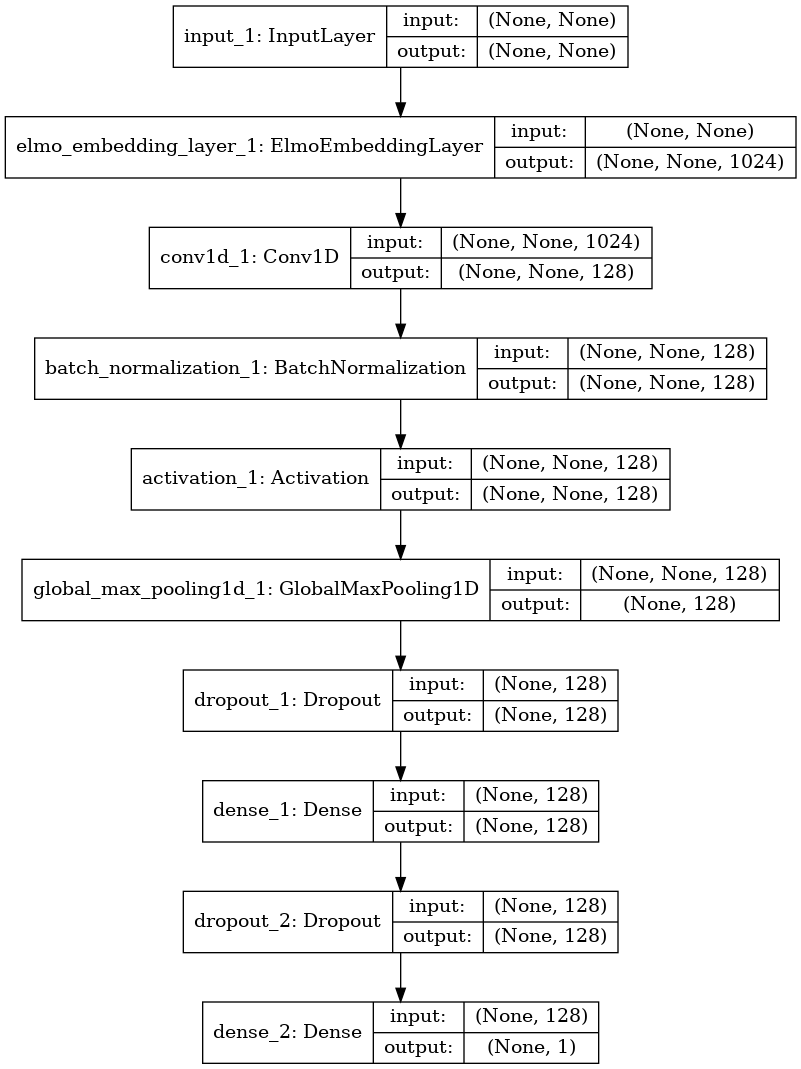
\includegraphics{elmo_model.png}
\end{frame}
